

\documentclass{beamer}
 
\usepackage[utf8]{inputenc}
 \usetheme{Madrid}
 \usecolortheme{beaver}
 \usefonttheme{structuresmallcapsserif}
 \usepackage{listings}
%Information to be included in the title page:


\title[Sensors and Actuators] %optional
{Sensors and Actuators}

\subtitle{An Overview}

\author[Dr. Joseph Kehoe] % (optional, for multiple authors)
{Joseph Kehoe\inst{1}}

\institute[IT Carlow] % (optional)
{
	\inst{1}%
	Department of Computing and Networking\\
	Institute of Technology Carlow
}

\date[ITC 2017] % (optional)
{CDD101, 2017}

\logo{
\includegraphics[height=1.5cm]{../../itcarlowlogo.png}}




 
 \AtBeginSection[]
 {
 	\begin{frame}
 		\frametitle{Table of Contents}
 		\tableofcontents[currentsection]
 	\end{frame}
 }
 
 
 
\begin{document}
 
\frame{\titlepage}
 
 
 
 \begin{frame}
 	\frametitle{Table of Contents}
 	\tableofcontents
 \end{frame}
 
 
 \section{Some Definitions}
 

  \begin{frame}
  	\frametitle{Sensors}
  	\begin{description}
  		\item[Sensor]A device which detects or measures a physical property and records, indicates, or otherwise responds to it
  	\end{description}
  	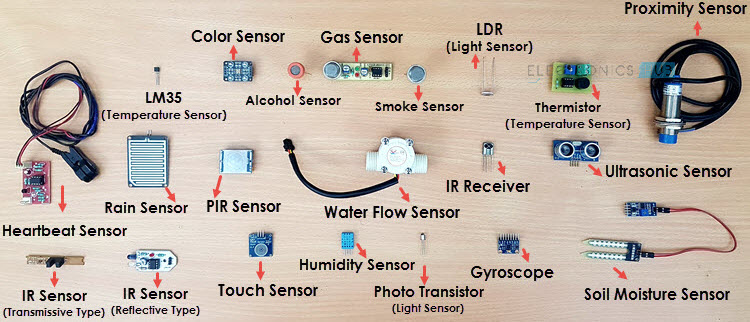
\includegraphics[height=4cm]{Types-of-Sensors.jpg}
  	
  \end{frame}

  \begin{frame}
  	\frametitle{Actuators}
  	\begin{description}
  		\item[Actuator] A component that is responsible for moving or controlling a mechanism or system; in simple terms, it is a "mover". An actuator requires a control signal and a source of energy. There are five main types of actuators – hydraulic, pneumatic, electrical, Thermal or Magnetic and Mechanical.
  	\end{description}
  	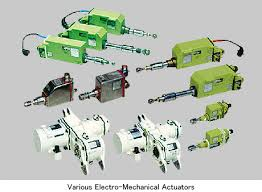
\includegraphics[height=3cm]{actuators.jpg}
  	
  \end{frame}

  \begin{frame}
  	\frametitle{UI}
\begin{itemize}
	\item 	Actuators and Sensors form the interface between a device and the world
	\item They determine what it can sense and what it can do
	\item i.e. How it interacts with us
	\item We must choose which to use based on purpose of device  
	\item This is an important part of device design
\end{itemize}	
  \end{frame}
  
  \begin{frame}
  	\frametitle{Measurement}
  	\begin{itemize}
  		\item 	Purpose of these sensors is to measure something
  		\item   Sometimes we can use them to directly measure something
  		\item but often we cannot measure what we want directly so we must use an indirect measurement
  		\item That is, measure something else that serves as an indicator for what we want to measure
  	\end{itemize}	
  	For each sensor on the next slide say what it measures directly and also give one example of something else it could be used to measure
  \end{frame}  
  
    \begin{frame}
    	\frametitle{Sensors Types}

    	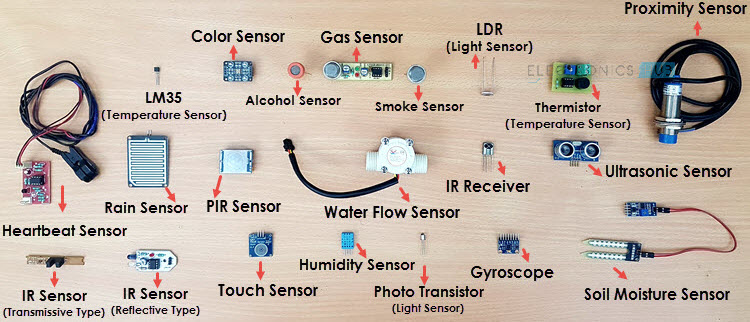
\includegraphics[height=5cm]{Types-of-Sensors.jpg}
    	
    \end{frame}
    
 \section{Case Studies}
\begin{frame}
	\frametitle{Smartphone}
	
     \begin{itemize}
     	\item List the sensors on a smartphone
     	\item Determine for each one two different things it can measure
     	\item Give one health based use case that employs smartphone sensors
     \end{itemize}
     

\end{frame}

  \begin{frame}
  	\frametitle{Grippy Bird}
  	
  	\begin{itemize}
  		\item Stroke patients sometimes need to develop their grip strength
  		\item Requires repetitive use of grip strengtheners
  		\item This is tedious and feedback is low
  		\item Add Sensor to gripping device
  		\item Turn repetitive work into a game: Grip causes bird to flap wings 
  		\item Rehab becomes fun and device/game records patient progress for medical staff
  	\end{itemize}
  		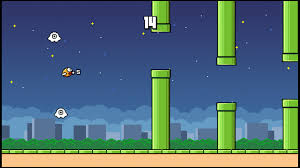
\includegraphics[height=3cm]{flappy.jpg}
  	
  \end{frame}

      \begin{frame}
      	\frametitle{Balance}
      	
      	\begin{itemize}
      		\item Stroke patients sometimes need to develop their balance/leg strength
      		\item Use Nintendo balance board
      		\item Use phone accelerometer
      		\item Add accelerometer to wearable device
      		\item Use XBox Kinect
      		\item Use treadmill 
      	\end{itemize}
      	
      	
      \end{frame}

        
\end{document}

